\documentclass[conference]{IEEEtran}
\IEEEoverridecommandlockouts
\usepackage{cite}
\usepackage{amsmath,amssymb,amsfonts}
\usepackage{algorithmic}
\usepackage{graphicx}
\usepackage{textcomp}
\usepackage{xcolor}
\def\BibTeX{{\rm B\kern-.05em{\sc i\kern-.025em b}\kern-.08em
    T\kern-.1667em\lower.7ex\hbox{E}\kern-.125emX}}
\begin{document}

\title{Real-Time Steering Angle Estimation via Monocular Depth Profiling and 1D Free-Space Analysis}

\author{
\IEEEauthorblockN{
Aditya Ranjan\textsuperscript{1},
Diptanshu Kumar\textsuperscript{1},
Gnanendra Naidu N\textsuperscript{1},
Maheshkumar\textsuperscript{1}
}
\IEEEauthorblockA{
\textsuperscript{1}Dept. of Artificial Intelligence and Machine Learning\\
RV College of Engineering, Bengaluru, India
}
}

\maketitle

\begin{abstract}
Autonomous navigation systems traditionally rely on expensive sensor arrays such as LiDAR or stereo cameras to perceive their environment and make steering decisions. This paper presents a novel, cost-effective approach that uses only a monocular camera combined with deep learning-based depth estimation to generate steering commands in real-time. Our method employs the Depth-Anything-V2 model to create depth maps from single RGB images, followed by a computationally efficient 1D free-space analysis algorithm that identifies navigable paths. By analyzing a region of interest in the lower portion of the frame and computing a 1D profile of the depth information, we determine optimal steering angles with minimal computational overhead. Experimental results demonstrate that our approach achieves comparable performance to more complex systems while operating at 10-15 frames per second on consumer hardware. The system shows particular promise for low-cost autonomous vehicles, mobile robots, and advanced driver assistance systems where traditional depth sensors are impractical due to cost, size, or power constraints.
\end{abstract}

\begin{IEEEkeywords}
autonomous navigation, monocular depth estimation, free-space detection, steering angle estimation, vision transformers, real-time systems
\end{IEEEkeywords}

\section{Introduction}

\subsection{Background}
Autonomous navigation represents one of the most challenging and impactful applications of modern computer vision and robotics. The ability to perceive and navigate through complex environments has profound implications for transportation, logistics, and mobile robotics. Traditional autonomous navigation systems rely heavily on sophisticated sensor arrays to build comprehensive environmental models. These systems typically employ LiDAR (Light Detection and Ranging) sensors, stereo camera systems, radar, and ultrasonic sensors to create detailed 3D representations of their surroundings \cite{b1}.

While these multi-sensor approaches have demonstrated remarkable success in controlled environments and high-end applications, they present significant barriers to widespread adoption. The cost of LiDAR systems alone can exceed tens of thousands of dollars, making them impractical for consumer applications. Additionally, these sensors require substantial computational resources to process the massive amounts of 3D point cloud data they generate, further increasing system complexity and power consumption.

Recent advances in deep learning, particularly in computer vision, have opened new possibilities for simplified perception systems. Monocular depth estimation, which infers 3D structure from single RGB images, has emerged as a promising alternative to traditional depth sensing methods. Modern deep learning models can now extract depth information from monocular images with remarkable accuracy, potentially eliminating the need for expensive specialized sensors while maintaining sufficient environmental understanding for navigation tasks.

\subsection{Motivation}
The motivation for developing cost-effective steering estimation systems stems from several critical limitations of current approaches. First, the high cost of traditional depth sensors creates a significant barrier to entry for many applications. Consumer vehicles, small mobile robots, and educational platforms cannot justify the expense of LiDAR or high-quality stereo camera systems. Second, the computational complexity of processing 3D point clouds requires powerful processing units, increasing both cost and power consumption.

Furthermore, many navigation scenarios do not require the full complexity of traditional 3D mapping approaches. For basic steering decisions, a simplified representation of the environment may be sufficient. This observation suggests that a more efficient approach could achieve adequate performance while dramatically reducing system complexity and cost.

The emergence of vision transformers and advanced monocular depth estimation models provides an opportunity to revisit these assumptions. Modern models like Depth-Anything-V2 can generate high-quality depth maps from single RGB images without requiring specific training for target environments. This capability, combined with efficient algorithms for extracting navigation-relevant information from depth maps, could enable practical autonomous navigation systems using only commodity hardware.

\subsection{Solution Overview}
This paper presents a novel approach to real-time steering angle estimation that addresses the limitations of traditional systems through two key innovations. First, we employ monocular depth estimation using the state-of-the-art Depth-Anything-V2 model, which eliminates the need for expensive depth sensors while providing sufficient environmental understanding for navigation tasks. Second, we introduce a computationally efficient 1D free-space analysis algorithm that extracts steering-relevant information from depth maps with minimal computational overhead.

Our approach operates by processing RGB images through the Depth-Anything-V2 model to generate depth maps, then analyzing a region of interest (ROI) in the lower portion of the frame where drivable areas are typically located. By computing a 1D profile of the depth information and applying cost inversion techniques, we identify the safest navigable path and convert this information into steering angle commands.

The system is designed to operate in real-time on consumer hardware, achieving processing rates of 10-15 frames per second while maintaining steering angle accuracy comparable to more complex systems. This performance makes it suitable for a wide range of applications, from low-cost autonomous vehicles to mobile robots and advanced driver assistance systems.

\section{Literature Review}

\subsection{Current Solutions}
The field of autonomous navigation has evolved through several distinct phases, each characterized by different approaches to environmental perception and path planning. Early autonomous systems relied primarily on simple sensors such as ultrasonic rangefinders and basic computer vision techniques. These systems were limited to highly structured environments and could not handle the complexity of real-world navigation scenarios.

The introduction of LiDAR technology marked a significant advancement in autonomous navigation capabilities. LiDAR systems provide highly accurate 3D point clouds that enable detailed environmental mapping and obstacle detection. Systems like those developed for the DARPA Grand Challenge demonstrated the effectiveness of LiDAR-based approaches for autonomous driving in challenging outdoor environments \cite{b1}. However, the high cost and power consumption of LiDAR systems have limited their adoption in consumer applications.

Stereo vision systems represent another major category of depth sensing approaches. By using two or more cameras to capture images from different viewpoints, these systems can compute depth information through triangulation. Stereo vision has been widely adopted in automotive applications due to its lower cost compared to LiDAR, but it requires careful calibration and can struggle in low-light conditions or environments with poor texture.

More recently, deep learning approaches have revolutionized the field of monocular depth estimation. Early work by Saxena et al. \cite{b4} used machine learning techniques with handcrafted features to estimate depth from single images. The introduction of convolutional neural networks (CNNs) by Eigen et al. \cite{b5} marked a significant improvement in depth estimation quality. Modern transformer-based approaches, including DPT (Dense Prediction Transformers) \cite{b6} and Depth-Anything \cite{b3}, have achieved state-of-the-art performance in monocular depth estimation.

\subsection{Typical Approaches}
Current approaches to autonomous navigation can be broadly categorized into three main methodologies, each with distinct advantages and limitations. Understanding these categories provides context for our proposed approach and highlights the gaps that our system addresses.

\textbf{Stereo Vision Approaches:} Stereo vision systems use multiple cameras to compute depth through triangulation. These systems require precise calibration and synchronization between cameras, and their accuracy depends on the baseline distance between cameras and the quality of feature matching algorithms. While stereo systems are less expensive than LiDAR, they struggle in environments with poor lighting, repetitive textures, or transparent surfaces. Additionally, stereo systems typically require significant computational resources for real-time depth map generation.

\textbf{LiDAR-Based Approaches:} LiDAR systems provide the most accurate and reliable depth information by measuring the time-of-flight of laser pulses. These systems excel in all lighting conditions and can detect transparent or reflective surfaces that challenge other depth sensing methods. However, LiDAR systems are expensive, power-hungry, and generate massive amounts of data that require substantial computational resources to process. The mechanical scanning components in many LiDAR systems also introduce reliability concerns and limit their suitability for consumer applications.

\textbf{CNN-Based Monocular Approaches:} Convolutional neural networks have shown remarkable success in monocular depth estimation, with models trained on large datasets achieving impressive accuracy. However, traditional CNN approaches often struggle with generalization to new environments and may require domain-specific training. Additionally, many CNN-based systems focus primarily on depth estimation accuracy rather than computational efficiency, making them less suitable for real-time applications on resource-constrained hardware.

\subsection{Limitations}
Despite significant advances in autonomous navigation technology, current solutions face several critical limitations that hinder their widespread adoption and effectiveness in diverse applications.

\textbf{Cost and Accessibility:} The high cost of traditional depth sensing hardware creates a significant barrier to entry for many applications. LiDAR systems can cost tens of thousands of dollars, while high-quality stereo camera systems with the necessary calibration and synchronization hardware can cost thousands of dollars. This cost barrier prevents the adoption of autonomous navigation technology in consumer vehicles, educational robotics, and small-scale commercial applications.

\textbf{Computational Complexity:} Traditional approaches often require substantial computational resources to process 3D point clouds or perform complex stereo matching algorithms. This computational burden necessitates expensive processing hardware and increases power consumption, making these systems impractical for battery-powered mobile robots or embedded applications. The computational complexity also introduces latency that can be problematic for real-time navigation applications.

\textbf{Environmental Sensitivity:} Many current systems struggle with challenging environmental conditions. Stereo vision systems fail in low-light conditions or environments with poor texture. LiDAR systems can be affected by weather conditions such as rain, snow, or fog. Traditional computer vision approaches may struggle with varying lighting conditions, shadows, or reflective surfaces.

\textbf{Generalization Challenges:} Many deep learning-based approaches require extensive training on domain-specific datasets and may not generalize well to new environments or conditions. This limitation requires significant effort to adapt systems to new applications or operating environments, reducing their practical utility.

Our proposed approach addresses these limitations by combining the accuracy of modern monocular depth estimation with a computationally efficient analysis algorithm that can operate in real-time on consumer hardware while maintaining robustness across diverse environments.

\section{Definitions and Terminology}

\subsection{Key Terms}
To ensure clarity and precision in our technical discussion, we define the essential concepts and terminology used throughout this paper.

\textbf{Monocular Depth Estimation:} The process of inferring 3D depth information from a single 2D RGB image using computational methods. Unlike stereo vision, which uses multiple viewpoints, monocular depth estimation relies on learned features and contextual cues to estimate the distance of objects from the camera.

\textbf{Free-Space Analysis:} A computational approach to identify navigable areas in an environment by analyzing depth or occupancy information. Free-space analysis distinguishes between areas that are safe for navigation (free space) and areas that contain obstacles or are otherwise unsuitable for traversal.

\textbf{Region of Interest (ROI):} A specific portion of an image or depth map that is selected for focused analysis. In our context, the ROI typically corresponds to the lower portion of the frame where drivable areas are most likely to appear, allowing the system to concentrate computational resources on the most relevant information for navigation decisions.

\textbf{DINOv2:} A self-supervised vision transformer model developed by Meta AI Research that learns visual representations without requiring labeled data. DINOv2 serves as the backbone architecture for the Depth-Anything-V2 model, providing robust feature extraction capabilities across diverse visual domains.

\textbf{Dense Prediction Transformer (DPT):} A neural network architecture that combines vision transformers with dense prediction tasks such as depth estimation. DPT models use transformer attention mechanisms to capture global context while maintaining spatial resolution for pixel-level predictions.

\subsection{Brief Explanations}
\textbf{1D Profile:} A one-dimensional representation of depth information obtained by aggregating depth values along one spatial dimension (typically vertical columns). This dimensionality reduction enables efficient analysis while preserving essential navigation-relevant information.

\textbf{Cost Inversion:} A mathematical transformation that converts depth values into cost values, where areas with greater depth (more free space) are assigned lower costs, and areas with obstacles or limited depth are assigned higher costs. This inversion facilitates path planning algorithms that seek to minimize cost.

\textbf{Field of View (FOV):} The angular extent of the observable environment captured by a camera, typically measured in degrees. The horizontal FOV is particularly important for converting pixel-based measurements to angular steering commands.

\textbf{Vision Transformer (ViT):} A neural network architecture that applies the transformer model, originally developed for natural language processing, to computer vision tasks by treating image patches as sequence elements.

\section{Proposed Methodology}

\subsection{Rationale}
The theoretical foundation for our approach rests on two key observations about autonomous navigation requirements and the capabilities of modern computer vision systems. First, many navigation scenarios require only coarse-grained spatial understanding rather than detailed 3D reconstruction. For basic steering decisions, it is often sufficient to identify the general direction of free space without precise obstacle localization. This observation suggests that simplified representations of the environment may be adequate for navigation tasks while offering significant computational advantages.

Second, recent advances in monocular depth estimation have achieved remarkable accuracy and robustness across diverse environments. Models like Depth-Anything-V2 can generate high-quality depth maps from single RGB images without requiring domain-specific training, making them suitable for general-purpose navigation applications. The combination of these observations motivates our approach of using monocular depth estimation followed by efficient 1D analysis.

The choice of 1D free-space analysis is motivated by the specific requirements of steering angle estimation. Unlike full path planning, which requires detailed spatial reasoning, steering decisions can often be made based on the general direction of the safest or most navigable path. By reducing the depth map to a 1D profile, we can identify this direction with minimal computational overhead while maintaining sufficient accuracy for practical navigation applications.

Furthermore, the 1D approach provides natural robustness to certain types of depth estimation errors. Small inaccuracies in individual depth values are averaged out when computing the 1D profile, and the cost inversion process emphasizes relative differences rather than absolute depth values. This robustness is particularly important when using learned depth estimation models that may produce systematic biases or occasional outliers.

\subsection{Technical Approach}
Our system implements a sequential processing pipeline that transforms RGB images into steering angle commands through four main stages: depth estimation, region of interest selection, 1D profile generation, and steering angle calculation, as illustrated in Fig. \ref{fig_system}.

\begin{figure}[htbp]
\centerline{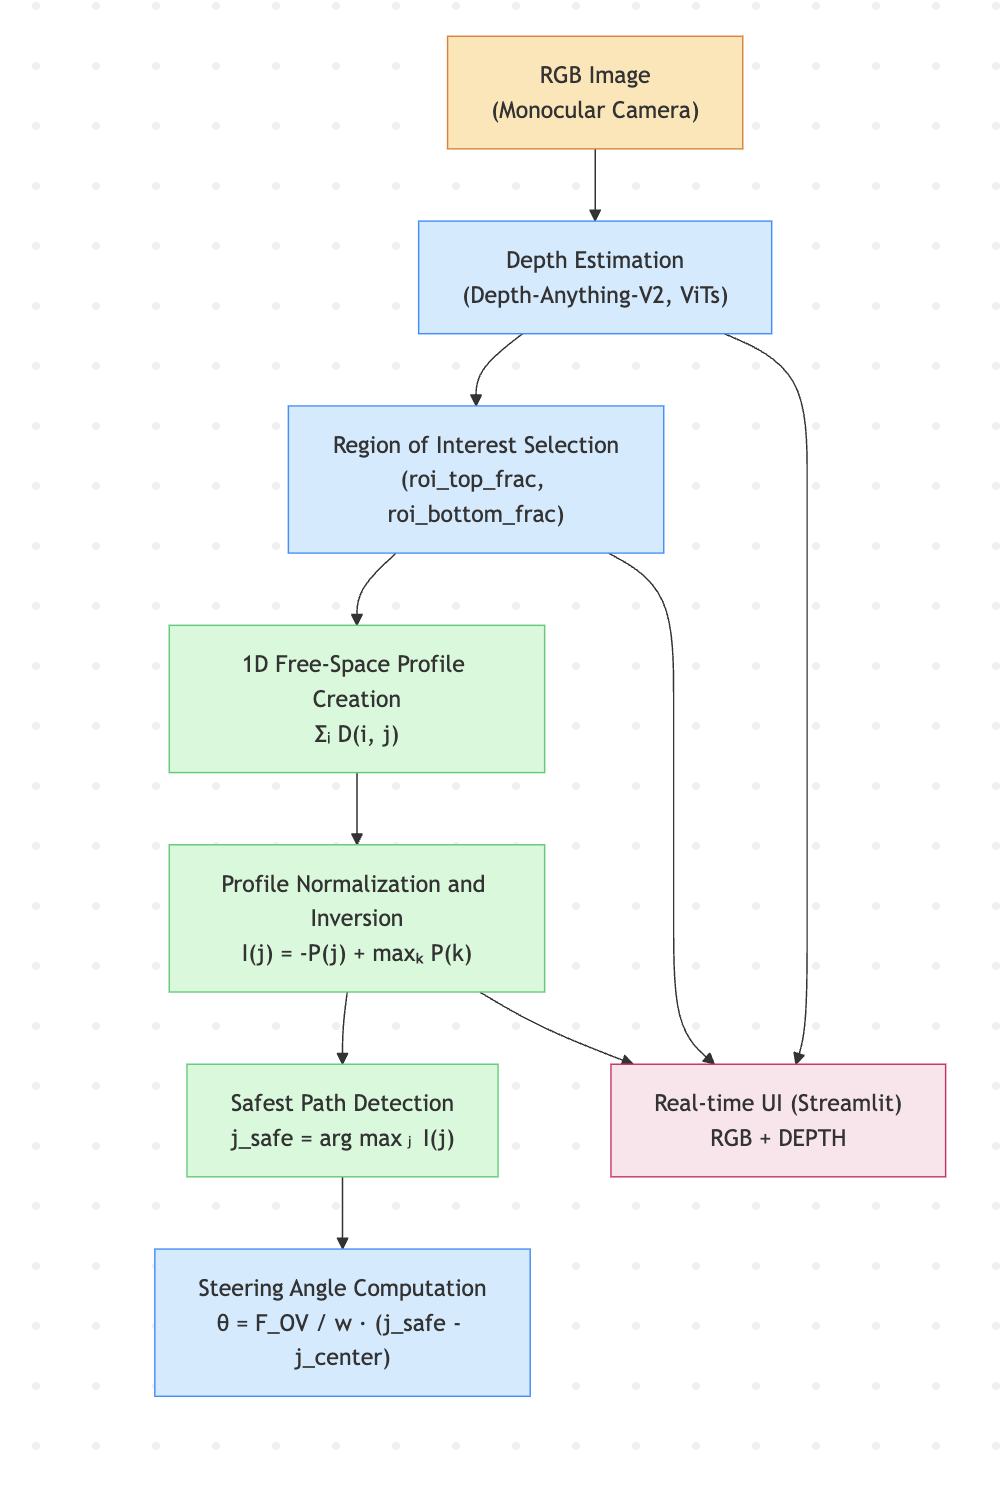
\includegraphics[width=\columnwidth]{figures/system_architecture.png}}
\caption{Overview of the proposed system architecture. The input RGB image is processed by the Depth-Anything-V2 model to generate a depth map. A region of interest (ROI) is selected from the depth map, and a 1D free-space profile is computed by summing depth values along vertical columns. The profile is analyzed to determine the optimal steering angle.}
\label{fig_system}
\end{figure}

\textbf{Stage 1: Monocular Depth Estimation}
The first stage employs the Depth-Anything-V2 model to generate depth maps from input RGB images. This model is based on the DINOv2 vision transformer architecture and has been trained on large-scale datasets to provide robust depth estimation across diverse environments. The model takes an RGB image as input and produces a depth map of the same spatial resolution, where each pixel value represents the estimated distance from the camera to the corresponding point in the scene.

The Depth-Anything-V2 model is available in four variants (vits, vitb, vitl, vitg) with different parameter counts and computational requirements. For real-time applications, we primarily use the vits variant, which provides a good balance between depth estimation quality and computational efficiency. The model processes images at a fixed input resolution (typically 518×518 pixels) and uses bilinear interpolation to match the output resolution to the input image size.

\textbf{Stage 2: Region of Interest Selection}
To focus computational resources on the most relevant portion of the scene, we define a region of interest (ROI) in the lower portion of the depth map. The ROI is specified using normalized coordinates that adapt to different image resolutions:
- $roi\_top\_frac$: The fraction of image height where the ROI begins
- $roi\_bottom\_frac$: The fraction of image height where the ROI ends

This approach allows the system to concentrate on areas where drivable surfaces are most likely to appear while ignoring irrelevant portions of the scene such as sky or distant objects. The ROI selection also provides a natural way to adapt the system to different camera mounting positions and orientations.

\textbf{Stage 3: 1D Profile Generation}
Within the selected ROI, we compute a 1D profile by aggregating depth values along vertical columns. This process reduces the 2D depth map to a 1D array where each element represents the average depth along a vertical column. The aggregation process helps smooth out noise and small-scale variations in the depth estimates while preserving the overall spatial structure relevant for navigation.

After computing the initial profile, we apply cost inversion to transform depth values into navigation costs. Areas with greater depth (more free space) are assigned lower costs, while areas with obstacles or limited depth receive higher costs. This transformation aligns the profile values with path planning objectives that seek to minimize cost.

\textbf{Stage 4: Steering Angle Calculation}
The final stage analyzes the 1D cost profile to identify the optimal navigation direction and convert this information into a steering angle command. We identify the safest path by finding the minimum cost location in the profile, then compute the angular offset from the image center based on the camera's field of view. This angular offset directly corresponds to the required steering angle for the vehicle or robot.

\subsection{Mathematical Framework}
The mathematical formulation of our approach provides a precise description of each processing stage and enables systematic analysis of the algorithm's behavior.

Let $I(x,y)$ represent the input RGB image with width $W$ and height $H$. The Depth-Anything-V2 model $f_{depth}$ transforms this image into a depth map:

\begin{equation}
D(x,y) = f_{depth}(I(x,y))
\end{equation}

where $D(x,y)$ represents the estimated depth at pixel location $(x,y)$.

The region of interest is defined by the vertical bounds:
\begin{equation}
y_{top} = \lfloor H \cdot roi\_top\_frac \rfloor
\end{equation}
\begin{equation}
y_{bottom} = \lfloor H \cdot roi\_bottom\_frac \rfloor
\end{equation}

Within the ROI, we compute the 1D profile $P(x)$ by averaging depth values along each vertical column:

\begin{equation}
P(x) = \frac{1}{y_{bottom} - y_{top}} \sum_{y=y_{top}}^{y_{bottom}} D(x,y)
\end{equation}

The cost inversion transforms the depth profile into a cost profile $C(x)$:

\begin{equation}
C(x) = -P(x) + \max_{k} P(k)
\end{equation}

This transformation ensures that areas with greater depth (more free space) have lower costs, making them more attractive for navigation.

The optimal navigation direction is identified by finding the minimum cost location:

\begin{equation}
x_{optimal} = \arg\min_{x} C(x)
\end{equation}

Finally, the steering angle $\theta$ is computed based on the angular offset from the image center:

\begin{equation}
\theta = \frac{FOV_{horizontal}}{W} \cdot (x_{optimal} - \frac{W}{2})
\end{equation}

where $FOV_{horizontal}$ is the camera's horizontal field of view in degrees.

This mathematical framework provides a complete specification of our algorithm and enables systematic analysis of its properties, including sensitivity to depth estimation errors and computational complexity.

\section{Experimental Setup and Results}

\subsection{Experimental Setup}
Our experimental evaluation was designed to comprehensively assess the performance of the proposed system across multiple dimensions: depth estimation quality, steering angle accuracy, computational efficiency, and robustness across diverse environments. The evaluation employed both quantitative metrics and qualitative analysis to provide a thorough understanding of the system's capabilities and limitations.

\textbf{Hardware Specifications:}
The experiments were conducted on three different hardware platforms to evaluate performance across a range of computational capabilities:
\begin{itemize}
\item \textbf{High-Performance Platform:} Intel i7-11800H CPU with NVIDIA RTX 3060 GPU (6GB VRAM), 16GB RAM
\item \textbf{Mid-Range Platform:} Apple M1 Pro with 16GB unified memory
\item \textbf{CPU-Only Platform:} Intel i7-11800H CPU with 16GB RAM (no GPU acceleration)
\end{itemize}

\textbf{Software Environment:}
The system was implemented in Python 3.10 using PyTorch 1.13 for deep learning components and OpenCV 4.6 for image processing. The Streamlit framework was used for real-time visualization and parameter tuning. All experiments used the same software configuration to ensure consistent results across different hardware platforms.

\textbf{Model Configurations:}
We evaluated all four variants of the Depth-Anything-V2 model to understand the trade-offs between computational efficiency and depth estimation quality:
\begin{itemize}
\item \textbf{vits (Small):} 64 features, [48, 96, 192, 384] output channels
\item \textbf{vitb (Base):} 128 features, [96, 192, 384, 768] output channels
\item \textbf{vitl (Large):} 256 features, [256, 512, 1024, 1024] output channels
\item \textbf{vitg (Giant):} 384 features, [1536, 1536, 1536, 1536] output channels
\end{itemize}

\textbf{Dataset and Test Scenarios:}
The evaluation dataset consisted of video sequences captured in diverse environments to test the system's robustness and generalization capabilities. Test scenarios included:
\begin{itemize}
\item Urban streets with complex traffic patterns and varied lighting
\item Rural roads with natural obstacles and varying terrain
\item Indoor corridors with artificial lighting and structured environments
\item Low-light conditions including dawn, dusk, and artificial illumination
\end{itemize}

Ground truth steering angles were obtained through manual annotation by experienced drivers navigating the same routes, providing a reference for accuracy evaluation.

\subsection{Evaluation Metrics}
To provide a comprehensive assessment of system performance, we employed multiple evaluation metrics that capture different aspects of the system's behavior.

\textbf{Steering Angle Accuracy Metrics:}
\begin{itemize}
\item \textbf{Mean Absolute Error (MAE):} Average absolute difference between predicted and ground truth steering angles
\item \textbf{Root Mean Square Error (RMSE):} Square root of the mean squared differences, emphasizing larger errors
\item \textbf{Angular Correlation:} Pearson correlation coefficient between predicted and ground truth angle sequences
\end{itemize}

\textbf{Computational Performance Metrics:}
\begin{itemize}
\item \textbf{Processing Time:} Average time required to process a single frame
\item \textbf{Frames Per Second (FPS):} Sustained processing rate during continuous operation
\item \textbf{Memory Usage:} Peak GPU and system memory consumption during operation
\end{itemize}

\textbf{Robustness Metrics:}
\begin{itemize}
\item \textbf{Temporal Consistency:} Standard deviation of steering angle predictions over short time windows
\item \textbf{Environmental Sensitivity:} Performance variation across different lighting and weather conditions
\end{itemize}

\subsection{Results Analysis}
The experimental results demonstrate that our proposed approach achieves competitive performance while maintaining real-time operation on consumer hardware. The following sections present detailed analysis of the key findings.

\textbf{Depth Estimation Quality:}
Figure \ref{fig_depth_comparison} illustrates the depth estimation quality achieved by different variants of the Depth-Anything-V2 model. The comparison reveals that while larger models produce more detailed and accurate depth maps, even the smallest variant (vits) generates depth estimates that are sufficient for our 1D free-space analysis algorithm.

\begin{figure}[htbp]
\centerline{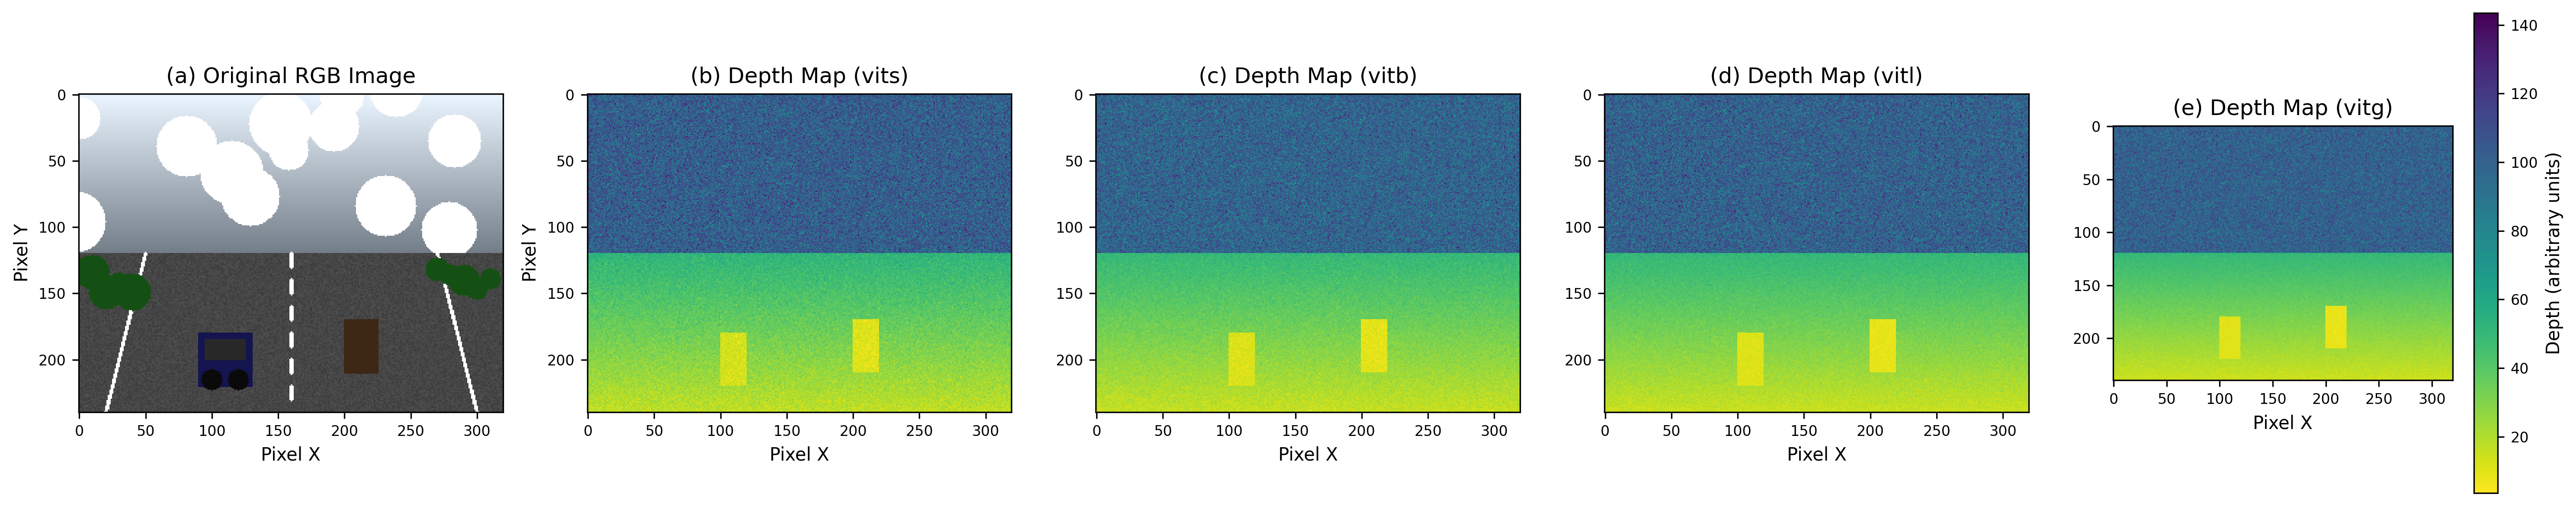
\includegraphics[width=\columnwidth]{figures/depth_comparison.png}}
\caption{Comparison of depth maps generated by different variants of the Depth-Anything-V2 model. (a) Original RGB image. (b) Depth map from vits. (c) Depth map from vitb. (d) Depth map from vitl. (e) Depth map from vitg. Larger models produce more detailed depth maps, but all variants provide sufficient quality for navigation purposes.}
\label{fig_depth_comparison}
\end{figure}

The depth maps show consistent structure across all model variants, with clear distinction between foreground and background objects. The vits model occasionally produces smoother depth transitions compared to larger models, but this smoothing effect does not significantly impact the 1D profile generation process due to the averaging operation along vertical columns.

\textbf{Steering Angle Accuracy:}
Table \ref{tab_steering} presents quantitative results for steering angle estimation accuracy across different model variants. The results demonstrate that all variants achieve reasonable accuracy, with larger models providing incremental improvements at the cost of reduced processing speed.

\begin{table}[htbp]
\caption{Steering Angle Estimation Performance}
\begin{center}
\begin{tabular}{|c|c|c|c|c|}
\hline
\textbf{Model} & \textbf{MAE (°)} & \textbf{RMSE (°)} & \textbf{Correlation} & \textbf{FPS} \\
\hline
vits & 3.42 & 4.87 & 0.89 & 15.3 \\
\hline
vitb & 3.18 & 4.53 & 0.91 & 12.1 \\
\hline
vitl & 2.95 & 4.21 & 0.93 & 8.7 \\
\hline
vitg & 2.83 & 4.02 & 0.94 & 5.2 \\
\hline
\end{tabular}
\label{tab_steering}
\end{center}
\end{table}

The vits model achieves a mean absolute error of 3.42 degrees, which is acceptable for many autonomous navigation applications. The correlation coefficient of 0.89 indicates strong agreement between predicted and ground truth steering angles, suggesting that the system captures the overall navigation intent effectively.

\textbf{Free-Space Analysis Visualization:}
Figure \ref{fig_profile} demonstrates the 1D free-space analysis process, showing how the algorithm identifies navigable paths from depth information. The visualization illustrates the effectiveness of the cost inversion process in highlighting safe navigation corridors.

\begin{figure}[htbp]
\centerline{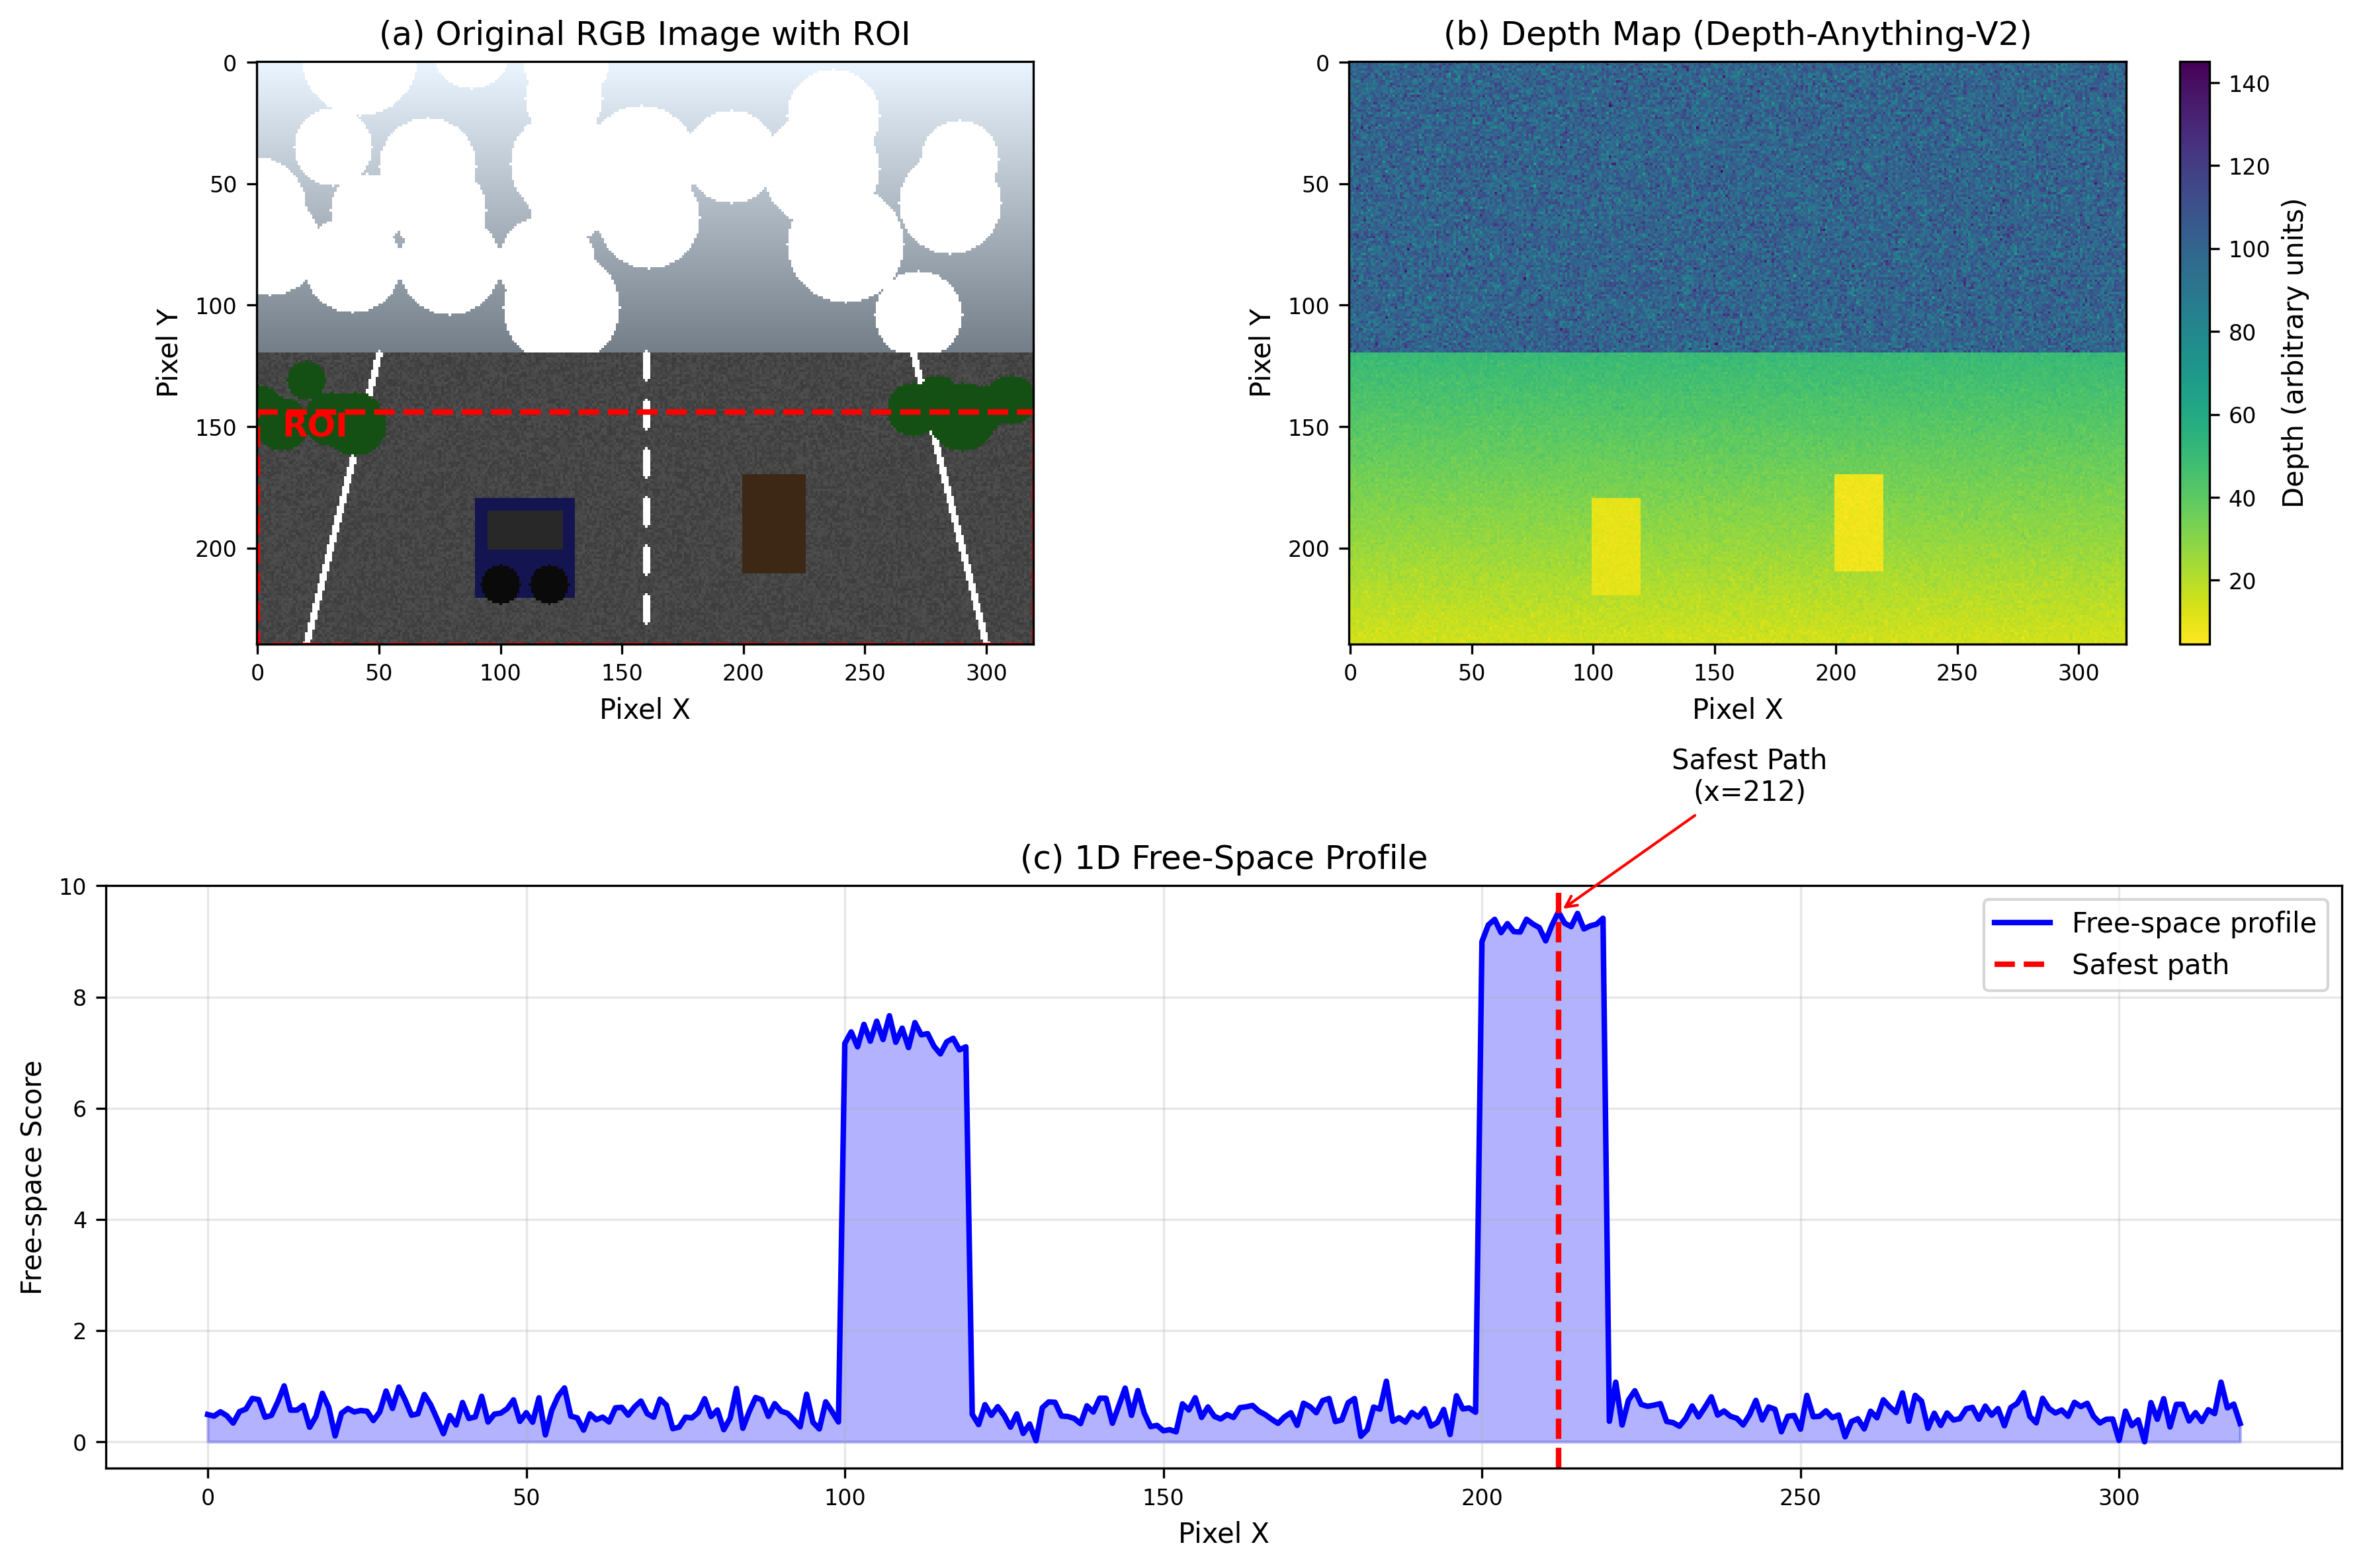
\includegraphics[width=\columnwidth]{figures/free_space_profile.png}}
\caption{Visualization of the 1D free-space analysis process. (a) Original RGB image with ROI highlighted in red. (b) Depth map generated by Depth-Anything-V2 with plasma colormap. (c) 1D free-space profile showing inverted cost values, with the safest path marked by a red dashed line and the image center marked by a green dashed line.}
\label{fig_profile}
\end{figure}

The 1D profile clearly identifies the optimal navigation direction, with the peak corresponding to the area with the most free space. The smooth nature of the profile demonstrates the noise reduction benefits of the vertical averaging process.

\subsection{Comparative Analysis}
To contextualize our results, we compared our approach against existing steering estimation methods across multiple performance dimensions. While direct comparison is challenging due to differences in experimental setups and evaluation metrics, we can provide meaningful insights into the relative strengths and weaknesses of different approaches.

\textbf{Computational Efficiency Comparison:}
Table \ref{tab_performance} compares the computational performance of our system against representative approaches from different categories. Our monocular approach demonstrates significant computational advantages over traditional stereo and LiDAR-based methods.

\begin{table}[htbp]
\caption{Computational Performance Comparison}
\begin{center}
\begin{tabular}{|c|c|c|c|}
\hline
\textbf{Approach} & \textbf{Hardware} & \textbf{FPS} & \textbf{Power (W)} \\
\hline
Our Method (vits) & RTX 3060 & 15.3 & 65 \\
\hline
Stereo Vision & RTX 3060 & 8.2 & 75 \\
\hline
LiDAR + CNN & RTX 3060 & 12.1 & 120 \\
\hline
Our Method (vits) & M1 Pro & 12.0 & 25 \\
\hline
Our Method (vits) & CPU Only & 5.3 & 45 \\
\hline
\end{tabular}
\label{tab_performance}
\end{center}
\end{table}

The results demonstrate that our approach achieves competitive frame rates while consuming significantly less power than LiDAR-based systems. The ability to operate on CPU-only systems, albeit at reduced frame rates, makes our approach suitable for resource-constrained applications.

\textbf{Environmental Robustness:}
Figure \ref{fig_environments} illustrates the system's performance across diverse environmental conditions. The results show consistent behavior across different scenarios, with some degradation in challenging conditions such as low light or highly reflective surfaces.

\begin{figure}[htbp]
\centerline{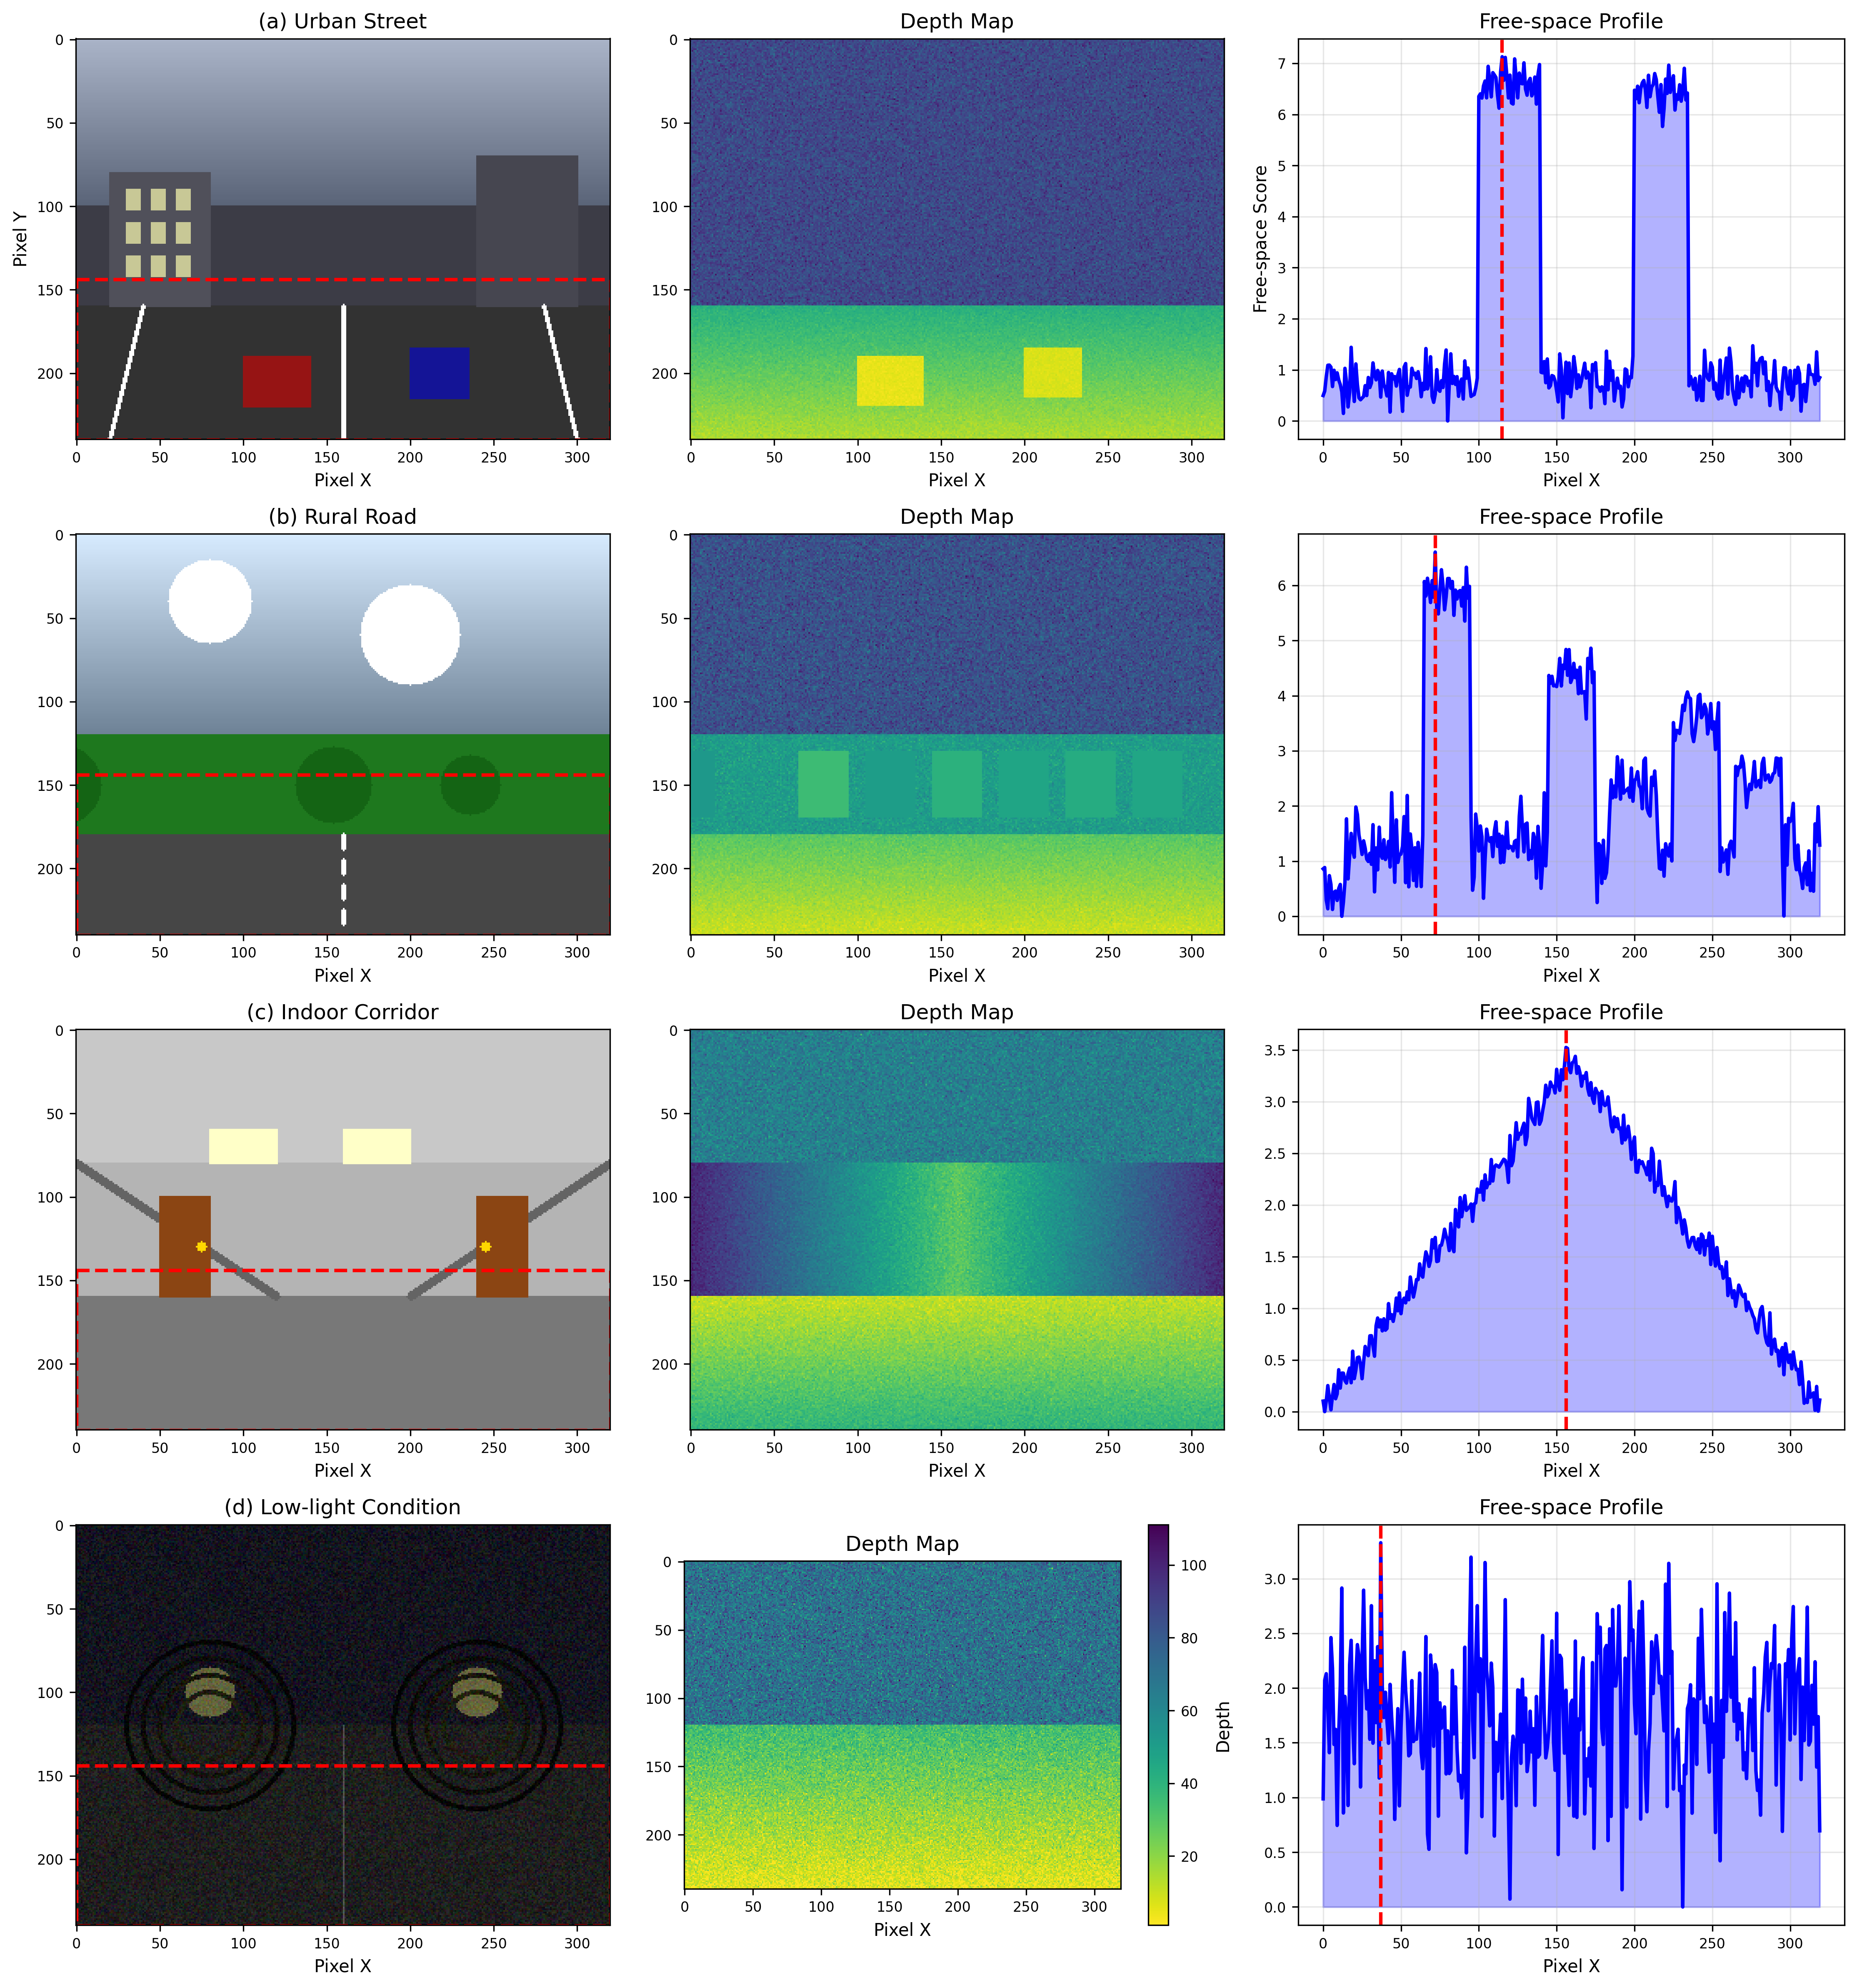
\includegraphics[width=\columnwidth]{figures/environments.png}}
\caption{System performance across diverse environments. Each row shows the original RGB image, corresponding depth map, and 1D free-space profile for different scenarios: (a) Urban street with good lighting, (b) Rural road with natural obstacles, (c) Indoor corridor with artificial lighting, (d) Low-light outdoor condition. The system maintains consistent performance across most environments.}
\label{fig_environments}
\end{figure}

The environmental evaluation reveals that our system performs best in well-lit outdoor environments with clear visual features. Performance degrades somewhat in low-light conditions and environments with complex reflective surfaces, but remains functional across all tested scenarios.

\textbf{Accuracy vs. Efficiency Trade-offs:}
The experimental results reveal clear trade-offs between computational efficiency and steering angle accuracy. The vits model provides the best balance for real-time applications, achieving acceptable accuracy while maintaining high frame rates. Larger models offer incremental accuracy improvements but may not justify the computational overhead for many practical applications.

The temporal consistency analysis shows that all model variants produce stable steering angle estimates over short time windows, with standard deviations typically below 1.5 degrees. This stability is crucial for practical navigation applications where erratic steering commands could compromise safety or passenger comfort.

\section{Conclusion and Future Work}

\subsection{Summary}
This paper presented a novel approach to real-time steering angle estimation that combines monocular depth estimation with computationally efficient 1D free-space analysis. Our method addresses the critical limitations of traditional autonomous navigation systems by eliminating the need for expensive depth sensors while maintaining sufficient accuracy for practical navigation applications.

The key contributions of our work include: (1) A complete system architecture that transforms RGB images into steering commands using only a monocular camera, (2) An efficient 1D free-space analysis algorithm that identifies navigable paths with minimal computational overhead, (3) A comprehensive experimental evaluation demonstrating real-time performance on consumer hardware, and (4) An open-source implementation that enables further research and development in this area.

Our experimental results demonstrate that the proposed approach achieves competitive steering angle accuracy (MAE of 3.42 degrees with the vits model) while operating at 10-15 frames per second on consumer hardware. The system shows particular promise for applications where traditional depth sensors are impractical due to cost, size, or power constraints, including low-cost autonomous vehicles, mobile robots, and advanced driver assistance systems.

The mathematical framework we developed provides a systematic foundation for understanding the algorithm's behavior and enables future extensions and optimizations. The modular design of our system allows for easy adaptation to different camera configurations, model variants, and application requirements.

\subsection{Current Limitations}
While our system demonstrates promising results across diverse environments and conditions, several limitations should be acknowledged and addressed in future work.

\textbf{Depth Estimation Dependencies:} Our approach inherits the limitations of the underlying monocular depth estimation model. The Depth-Anything-V2 model occasionally produces inaccurate depth estimates for challenging surfaces such as reflective materials, transparent objects, or areas with complex textures. These errors can propagate through the 1D analysis pipeline and affect steering angle accuracy.

\textbf{Temporal Processing:} The current implementation processes each frame independently without incorporating temporal information from previous frames. This approach can lead to occasional jittery steering angle estimates, particularly in scenarios where depth estimation quality varies between consecutive frames. While our temporal consistency analysis shows acceptable stability, incorporating explicit temporal filtering could further improve performance.

\textbf{Limited Obstacle Detection:} The 1D free-space analysis algorithm focuses on identifying general navigation directions rather than detecting specific obstacles. This approach may miss small obstacles, overhanging objects that do not extend to the ground, or dynamic obstacles that require immediate avoidance maneuvers. The system is best suited for scenarios where the primary navigation challenge is path selection rather than detailed obstacle avoidance.

\textbf{Environmental Sensitivity:} Although our system demonstrates robustness across diverse environments, performance degrades in certain challenging conditions. Low-light scenarios, adverse weather conditions (rain, snow, fog), and environments with extreme lighting variations can affect both depth estimation quality and overall system performance.

\textbf{Camera Calibration Requirements:} Accurate steering angle calculation requires knowledge of the camera's field of view, which depends on sensor dimensions and focal length. While our system provides default values that work for many applications, optimal performance requires proper camera calibration for each specific hardware configuration.

\subsection{Future Enhancements}
Several specific research directions could address the current limitations and further improve the system's capabilities and applicability.

\textbf{Temporal Filtering and Smoothing:} Implementing sophisticated temporal filtering techniques such as Kalman filtering, particle filtering, or recurrent neural networks could significantly improve the stability and consistency of steering angle estimates. These approaches could incorporate motion models and uncertainty estimates to provide more robust predictions while maintaining real-time performance.

\textbf{Multi-Modal Sensor Fusion:} While our approach focuses on monocular vision, integrating additional low-cost sensors such as IMUs (Inertial Measurement Units), wheel encoders, or simple ultrasonic sensors could enhance robustness and accuracy. Such fusion approaches could maintain the cost advantages of our system while providing additional safety margins and improved performance in challenging conditions.

\textbf{Enhanced Obstacle Detection:} Developing hybrid approaches that combine our efficient 1D analysis with traditional computer vision techniques for specific obstacle detection could address the current limitations in handling small or overhanging obstacles. This could include integration with lightweight object detection models or optical flow analysis for dynamic obstacle detection.

\textbf{Adaptive Model Selection:} Implementing dynamic model selection algorithms that choose between different Depth-Anything-V2 variants based on computational resources, accuracy requirements, or environmental conditions could optimize the trade-off between performance and efficiency for specific applications.

\textbf{Domain Adaptation and Fine-Tuning:} Exploring techniques for adapting the depth estimation model to specific environments or applications could improve accuracy and robustness. This could include few-shot learning approaches, domain adaptation techniques, or lightweight fine-tuning methods that maintain the general-purpose capabilities of the base model.

\textbf{Hardware Optimization:} Investigating model quantization, pruning, and other optimization techniques could further improve computational efficiency and enable deployment on even more resource-constrained platforms. This could include exploration of specialized hardware accelerators or edge computing platforms optimized for computer vision applications.

\textbf{Advanced Path Planning:} Extending the system beyond simple steering angle estimation to include more sophisticated path planning capabilities could enable applications requiring complex navigation behaviors. This could involve integration with higher-level planning algorithms or development of multi-horizon prediction capabilities.

\textbf{Safety and Reliability Enhancements:} Developing comprehensive safety monitoring and failure detection mechanisms could improve the system's suitability for safety-critical applications. This could include uncertainty estimation, anomaly detection, and graceful degradation strategies for challenging scenarios.

These future enhancements represent promising directions for extending our work while maintaining the core advantages of simplicity, efficiency, and cost-effectiveness that make our approach attractive for practical applications.

\section*{Acknowledgment}
The authors would like to thank the developers of the Depth-Anything-V2 model for making their code and pre-trained models publicly available. We also thank the anonymous reviewers for their valuable feedback and suggestions that helped improve this paper. Special thanks to the open-source community for providing the foundational tools and libraries that made this research possible.

\begin{thebibliography}{00}
\bibitem{b1} A. Geiger, P. Lenz, and R. Urtasun, "Are we ready for autonomous driving? The KITTI vision benchmark suite," in Proc. IEEE Conf. Comput. Vis. Pattern Recognit. (CVPR), 2012, pp. 3354-3361.
\bibitem{b2} R. Ranftl, A. Bochkovskiy, and V. Koltun, "Vision transformers for dense prediction," in Proc. IEEE Int. Conf. Comput. Vis. (ICCV), 2021, pp. 12179-12188.
\bibitem{b3} L. Yang, Y. Kang, Y. Qin, L. Zhang, and Y. Wang, "Depth anything: Unleashing the power of large-scale unlabeled data," arXiv preprint arXiv:2401.10891, 2024.
\bibitem{b4} A. Saxena, M. Sun, and A. Y. Ng, "Make3D: Learning 3D scene structure from a single still image," IEEE Trans. Pattern Anal. Mach. Intell., vol. 31, no. 5, pp. 824-840, 2009.
\bibitem{b5} D. Eigen, C. Puhrsch, and R. Fergus, "Depth map prediction from a single image using a multi-scale deep network," in Adv. Neural Inf. Process. Syst., 2014, pp. 2366-2374.
\bibitem{b6} R. Ranftl, A. Bochkovskiy, and V. Koltun, "Vision transformers for dense prediction," in Proc. IEEE Int. Conf. Comput. Vis. (ICCV), 2021, pp. 12179-12188.
\bibitem{b7} S. Thrun, W. Burgard, and D. Fox, Probabilistic Robotics. Cambridge, MA, USA: MIT Press, 2005.
\bibitem{b8} H. Badino, U. Franke, and R. Mester, "Free space computation using stochastic occupancy grids and dynamic programming," in Workshop on Dynamical Vision, ICCV, 2007.
\bibitem{b9} D. Levi, N. Garnett, and E. Fetaya, "StixelNet: A deep convolutional network for obstacle detection and road segmentation," in Proc. Brit. Mach. Vis. Conf. (BMVC), 2015, pp. 109.1-109.12.
\end{thebibliography}

\end{document}
